\chapter{Astrofísica}\label{ch:b3:astrophysics}

% Provenance (not for print): the astrophysics option offered across the
% surveyed third-year curricula, built here as a capstone that reuses the
% whole volume (Fermi gas -> white dwarfs, nuclear -> stellar burning,
% Planck law -> CMB, Saha -> recombination).

Todo capítulo deste livro vinha ensaiando para este. As estrelas
são bolas de gás autogravitantes regidas pela hidrostática do volume do
primeiro ano, acesas pelo tunelamento do \cref{ch:b3:nuclear-physics} e
brilhando pela \omterm{thm:b3:photons-phonons:planck}{lei de Planck} do \cref{ch:b3:photons-phonons}; as estrelas
mortas são os gases de Fermi degenerados do
\cref{ch:b3:quantum-statistics} do tamanho de cidades;
e o próprio universo é um sistema térmico em resfriamento cuja
foto de bebê --- a radiação de fundo em micro-ondas --- é o corpo negro
mais perfeito já medido. Este capítulo de fecho reúne o volume
inteiro no maior laboratório possível: como as estrelas vivem, como
morrem, o que deixam para trás e como o universo em expansão
que as contém começou como física que já fizemos.

\section{Uma estrela é um equilíbrio}

\begin{proposition}[Equilíbrio hidrostático]\label{prop:b3:astrophysics:hydrostatic}
\index{equilíbrio hidrostático (estelar)}\index{estrutura estelar}
Uma estrela nem desaba nem se dispersa: em cada raio, o
gradiente de pressão carrega o peso do gás acima. Para a
massa $m(r)$ dentro do raio $r$,
\[
\frac{\dd P}{\dd r} = -\frac{Gm(r)\rho(r)}{r^2} .
\]
Estimado para todo o Sol, $P_{\text{c}} \sim GM^2/R^4 \sim
\qty{e15}{Pa}$ e, pela lei dos gases ideais, $T_{\text{c}} \sim
10^7\,\unit{K}$ (\cref{exo:b3:astrophysics:1}) --- precisamente a
temperatura em que os prótons do \cref{exo:b3:nuclear-physics:11}
começam a tunelar. Isso não é coincidência, e sim um termostato: uma
estrela \emph{tem} de se contrair e esquentar até o núcleo dela acender,
e a fusão então segura o equilíbrio por milhões a bilhões de anos. As
estrelas têm capacidade térmica negativa --- perdem energia, contraem,
ficam \emph{mais quentes} (\cref{exo:b3:astrophysics:5}) --- e é por isso
que a gravidade sempre vence no fim.
\end{proposition}

\begin{proof}
Uma casca $[r, r + \dd r]$ de área $A$ sente a pressão $P(r)A$ vinda
de baixo, $P(r + \dd r)A$ de cima, e o peso $g\rho A\,\dd r$
com $g = Gm(r)/r^2$ (só a massa interior puxa, pelo teorema de
Gauss para a gravidade). O equilíbrio dos três dá a
equação enunciada.
\end{proof}

\begin{omfigure}
\begin{tikzpicture}[scale=1.0]
  \fill[omExo!14] (0,0) circle (2.2);
  \fill[omExo!30] (0,0) circle (1.15);
  \draw[omDef, thick] (0,0) circle (2.2);
  \draw[omDef!60] (0,0) circle (1.15);
  \node[font=\scriptsize, align=center] at (0,0)
    {núcleo\\$10^7\,\unit{K}$: fusão};
  % pressure arrows outward
  \foreach \ang in {25,115,205,295}
    \draw[->, omThm, thick] (\ang:1.25) -- (\ang:1.8);
  \node[omThm, font=\scriptsize, anchor=west] at (2.5,0.85)
    {a pressão empurra para fora};
  % gravity arrows inward
  \foreach \ang in {70,160,250,340}
    \draw[->, omDef, thick] (\ang:2.75) -- (\ang:2.3);
  \node[omDef, font=\scriptsize, anchor=west] at (2.5,-0.85)
    {a gravidade puxa para dentro};
\end{tikzpicture}

{\small Uma estrela, desenhada como o diagrama de corpo livre dela. A
fusão alimenta a pressão que carrega o próprio peso da estrela; as duas
forças negociam por dez bilhões de anos --- e todo destino estelar deste
capítulo é o que acontece quando uma delas fica sem argumentos.}
\end{omfigure}

\section{As vidas das estrelas}

\begin{definition}[O diagrama de Hertzsprung--Russell]\label{def:b3:astrophysics:hr}
\index{diagrama de Hertzsprung--Russell}\index{sequência principal}
Trace as estrelas por temperatura superficial (as quentes à
\emph{esquerda}, por convenção) contra luminosidade, ambas vindas das
leis do corpo negro do \cref{ch:b3:photons-phonons}, e elas se recusam a
se espalhar: noventa por cento se amontoam na \emph{sequência
principal}, a faixa diagonal das queimadoras de hidrogênio, ordenadas
puramente pela massa --- mais pesada significa mais quente \emph{e}
desproporcionalmente mais brilhante ($L \propto M^{3.5}$), e portanto de
vida mais curta ($t \propto M/L \propto M^{-2.5}$:
\cref{exo:b3:astrophysics:4}). Fora da faixa vivem as
exceções e os finais do gráfico: as \emph{gigantes} frias, porém enormes
(canto superior direito), e as \emph{\omterm{ex:b3:quantum-statistics:dwarf}{anãs brancas}} quentes, porém
minúsculas (canto inferior esquerdo) --- porque, a temperatura fixa, por
$L = 4\pi R^2\sigma T^4$, a luminosidade é uma medida de \emph{tamanho}.
O diagrama HR não é um mapa de espécies, e sim de \emph{idades}: o ponto
de uma estrela vaga por ele à medida que o combustível dela se esgota.
\end{definition}

\begin{omfigure}
\begin{tikzpicture}
  \begin{axis}[omaxis, axis x line=bottom, axis y line=left,
    width=9.8cm, height=6.8cm, xmin=0, xmax=10, ymin=-4.6, ymax=6.4,
    xlabel={temperatura superficial (quente $\to$ fria)},
    ylabel={$\log_{10}(L/L_\odot)$},
    xlabel style={at={(axis description cs:0.5,-0.08)}, anchor=north},
    xtick=\empty, ytick={-4,-2,0,2,4,6}, clip=false]
    % main sequence band
    \addplot[omDef, line width=5pt, opacity=0.28, domain=0.6:9.4]
      {5.0 - 1.05*x};
    \addplot[omDef, thick, domain=0.6:9.4] {5.0 - 1.05*x};
    % sun
    \fill[omExo] (axis cs:4.76,0) circle (2pt);
    \node[omExo, font=\scriptsize, anchor=north east] at (axis cs:4.6,-0.4)
      {Sol};
    % giants
    \fill[omThm!25] (axis cs:8.1,3.4) ellipse (1.35 and 1.0);
    \node[omThm, font=\scriptsize] at (axis cs:8.1,3.4) {gigantes};
    % white dwarfs
    \fill[gray!25] (axis cs:2.6,-3.2) ellipse (1.5 and 0.75);
    \node[font=\scriptsize] at (axis cs:2.6,-3.2) {anãs brancas};
    \node[omDef, font=\scriptsize, rotate=-38, anchor=south] at
      (axis cs:2.6,2.5) {sequência principal};
  \end{axis}
\end{tikzpicture}

{\small O \omterm{def:b3:astrophysics:hr}{diagrama de Hertzsprung--Russell}. A \omterm{def:b3:astrophysics:hr}{sequência principal} é a
faixa que queima hidrogênio, uma escada de massas lida do alto à
esquerda (azuis, esbanjadoras, mortas em milhões de anos) até a base à
direita (vermelhas, frugais, sobrevivendo ao universo até aqui). As
gigantes e as \omterm{ex:b3:quantum-statistics:dwarf}{anãs brancas} não são esquisitices, e sim capítulos: a
mesma estrela visita as três regiões.}
\end{omfigure}

\begin{remark}[Como as estrelas envelhecem e o que deixam]\label{rem:b3:astrophysics:evolution}
\index{gigante vermelha}\index{supernova}\index{nucleossíntese (estelar)}
Quando o hidrogênio do núcleo se esgota, a lógica do termostato se
repete: o núcleo se contrai e esquenta, o hélio acende (fundindo-se em
carbono e oxigênio), o envelope incha cem vezes --- uma \omterm{rem:b3:astrophysics:evolution}{gigante vermelha}.
Uma estrela como o Sol para por aí: ela solta o envelope e se aposenta
como \omterm{ex:b3:quantum-statistics:dwarf}{anã branca}. Uma estrela acima de $\approx8M_\odot$ continua acendendo
combustíveis novos em cascas de cebola até o núcleo ser de \emph{ferro} ---
o cume da \cref{prop:b3:nuclear-physics:binding}, do qual fusão alguma
devolve energia. O núcleo morto desaba num segundo; o
ricochete e a enxurrada de neutrinos explodem a estrela: uma
\emph{supernova}, que por um instante ofusca a galáxia dela, forja os
elementos além do ferro por captura de nêutrons e espalha tudo
nas nuvens que constroem a próxima geração de estrelas e
planetas. O cálcio dos seus ossos e o ferro do seu sangue
fizeram este caminho (\cref{pb:b3:astrophysics:1}): a química é
astrofísica reciclada.
\end{remark}

\section{Os cadáveres: a matéria nos limites dela}

\begin{proposition}[Anãs brancas e estrelas de nêutrons]\label{prop:b3:astrophysics:compact}
\index{anã branca}\index{estrela de nêutrons}\index{massa de Chandrasekhar}\index{buraco negro}\index{raio de Schwarzschild}
O que segura uma estrela que não queima mais? A mecânica quântica. Uma
\emph{\omterm{ex:b3:quantum-statistics:dwarf}{anã branca}} é uma massa solar de carbono e oxigênio escorada
pela \emph{\omterm{thm:b3:quantum-statistics:fermi}{pressão de degenerescência}} eletrônica dela --- a pressão de
Fermi a $T = 0$ do \cref{ch:b3:quantum-statistics} --- no tamanho
da Terra e a uma tonelada por colher de chá. O sustento de Pauli tem um
teto: acima da \emph{\omterm{prop:b3:astrophysics:compact}{massa de Chandrasekhar}} $M_{\text{Ch}}
\approx 1.4\,M_\odot$, os elétrons ficam relativísticos e a
pressão perde a corrida (um resultado que enunciamos, não deduzimos). Além
dele, os elétrons são esmagados dentro dos prótons e se forma uma
\emph{\omterm{prop:b3:astrophysics:compact}{estrela de nêutrons}}: degenerescência de nêutrons mais repulsão
nuclear segurando $\sim1.4\,M_\odot$ em uma dúzia de quilômetros à
densidade nuclear da \cref{def:b3:nuclear-physics:nuclide} --- um
núcleo do tamanho de uma cidade, girando até milissegundos e emitindo
feixe como um farol (um \emph{pulsar}). E além de cerca de $3\,M_\odot$
nada conhecido resiste: a estrela cai para dentro do raio em que a
fuga exige a velocidade da luz,
\[
R_{\text{s}} = \frac{2GM}{c^2}
\qquad (\qty{3}{km}\text{ por massa solar}) ,
\]
um \emph{\omterm{prop:b3:astrophysics:compact}{buraco negro}} --- a palavra final da gravidade, e a soleira da
relatividade geral, um volume além deste.
\end{proposition}
\admitted

\begin{omfigure}
\begin{tikzpicture}[scale=1.0]
  % log-scale size ladder
  \draw[omDef, fill=omExo!18, thick] (0,0) circle (1.9);
  \node[font=\scriptsize, align=center] at (0,-2.35)
    {Sol\\$7\times10^5$ km};
  \draw[omDef, fill=omDef!15, thick] (4.4,0) circle (0.55);
  \node[font=\scriptsize, align=center] at (4.4,-2.35)
    {anã branca\\$\sim\qty{7000}{km}$};
  \draw[omThm, fill=omThm!18, thick] (7.3,0) circle (0.16);
  \node[font=\scriptsize, align=center] at (7.3,-2.35)
    {estrela de nêutrons\\$\sim\qty{12}{km}$};
  \fill (9.7,0) circle (0.06);
  \node[font=\scriptsize, align=center] at (9.7,-2.35)
    {buraco negro\\$R_{\text{s}} \sim \qty{4}{km}$};
  \node[font=\scriptsize, gray, anchor=south, align=center] at (4.85,1.55)
    {massa parecida, gravidade cada vez mais feroz\\(tamanhos fora de escala)};
\end{tikzpicture}

{\small Uma massa solar, quatro tamanhos. A pressão térmica segura o
Sol; a degenerescência eletrônica, a \omterm{ex:b3:quantum-statistics:dwarf}{anã branca}; a de nêutrons, a
\omterm{prop:b3:astrophysics:compact}{estrela de nêutrons}; nada segura o \omterm{prop:b3:astrophysics:compact}{buraco negro}. Cada passo multiplica a
gravidade superficial por uns dez mil --- e a física necessária
para ficar de pé sobre ela.}
\end{omfigure}

\section{O universo em expansão}

\begin{definition}[A lei de Hubble e o começo quente]\label{def:b3:astrophysics:hubble}
\index{lei de Hubble}\index{radiação cósmica de fundo em micro-ondas}\index{nucleossíntese do Big Bang}
Toda galáxia distante se afasta, a uma velocidade proporcional à distância:
\[
v = H_0d , \qquad H_0 \approx \qty{70}{km/s}
\text{ por megaparsec} .
\]
Isso não é uma explosão \emph{para dentro} do espaço, e sim uma expansão
\emph{do} espaço --- rode ao contrário e tudo já foi
denso e quente: $1/H_0 \approx 14$ bilhões de anos atrás
(\cref{exo:b3:astrophysics:9}). O universo primitivo é este livro
repassado em alta velocidade. Com um segundo, ele é uma sopa de
partículas de \unit{MeV} (\cref{ch:b3:particle-physics}); nos primeiros
minutos, o \cref{ch:b3:nuclear-physics} corre solto e congela
\emph{um quarto de hélio em massa} --- previsto por um fator de
Boltzmann, observado em toda parte
(\cref{exo:b3:astrophysics:11}). Aos 380\,000 anos e
\qty{3000}{K}, a \omterm{prop:b3:grand-canonical:saha}{equação de Saha}
(\cref{prop:b3:grand-canonical:saha}) deixa os elétrons enfim se
assentarem sobre os prótons; a névoa se dissipa, e essa luz espalhada
pela última vez --- esticada por um fator mil pela expansão --- chega
hoje como a \emph{radiação cósmica de fundo em micro-ondas}: um espectro
de Planck a \qty{2.725}{K} (\cref{ch:b3:photons-phonons}), a fotografia
mais antiga que existe. O que a imagem também mostra: as galáxias giram e
se agrupam como se guiadas por \emph{\omterm{rem:b3:particle-physics:higgs}{matéria escura}} que detector algum
capturou, e a expansão \emph{acelera} sob uma \emph{energia escura}
que ninguém explicou --- os noventa e cinco por cento do orçamento
que este livro ainda não sabe escrever.
\end{definition}

\begin{omfigure}
\begin{tikzpicture}
  \begin{axis}[omaxis, axis x line=bottom, axis y line=left,
    width=9.6cm, height=5.8cm, xmin=0, xmax=105, ymin=0, ymax=8.4,
    xlabel={distância (\unit{Mpc})},
    ylabel={velocidade de recessão ($10^3\,\unit{km/s}$)},
    xlabel style={at={(axis description cs:0.5,-0.1)}, anchor=north},
    xtick={25,50,75,100}, ytick={2,4,6,8}, clip=true]
    \addplot[omDef, thick, domain=0:103] {0.07*x};
    \addplot[only marks, mark=*, mark size=1.4pt, omThm]
      coordinates {(9,0.75) (17,1.05) (24,1.85) (31,2.0) (39,2.9)
        (46,3.05) (54,3.95) (61,4.1) (69,5.05) (76,5.15)
        (84,6.05) (91,6.2) (98,7.0)};
    \node[omDef, font=\scriptsize, anchor=north west] at (axis cs:57,3.6)
      {inclinação $H_0$};
  \end{axis}
\end{tikzpicture}

{\small A \omterm{def:b3:astrophysics:hubble}{lei de Hubble}: velocidade de recessão contra distância, com
cada ponto uma galáxia (velocidades vindas de desvios Doppler,
\cref{ch:b3:relativistic-kinematics}; distâncias, de velas-padrão). A
inclinação é $H_0$; o inverso dela é, grosso modo, a idade
do universo.}
\end{omfigure}

\begin{omfigure}
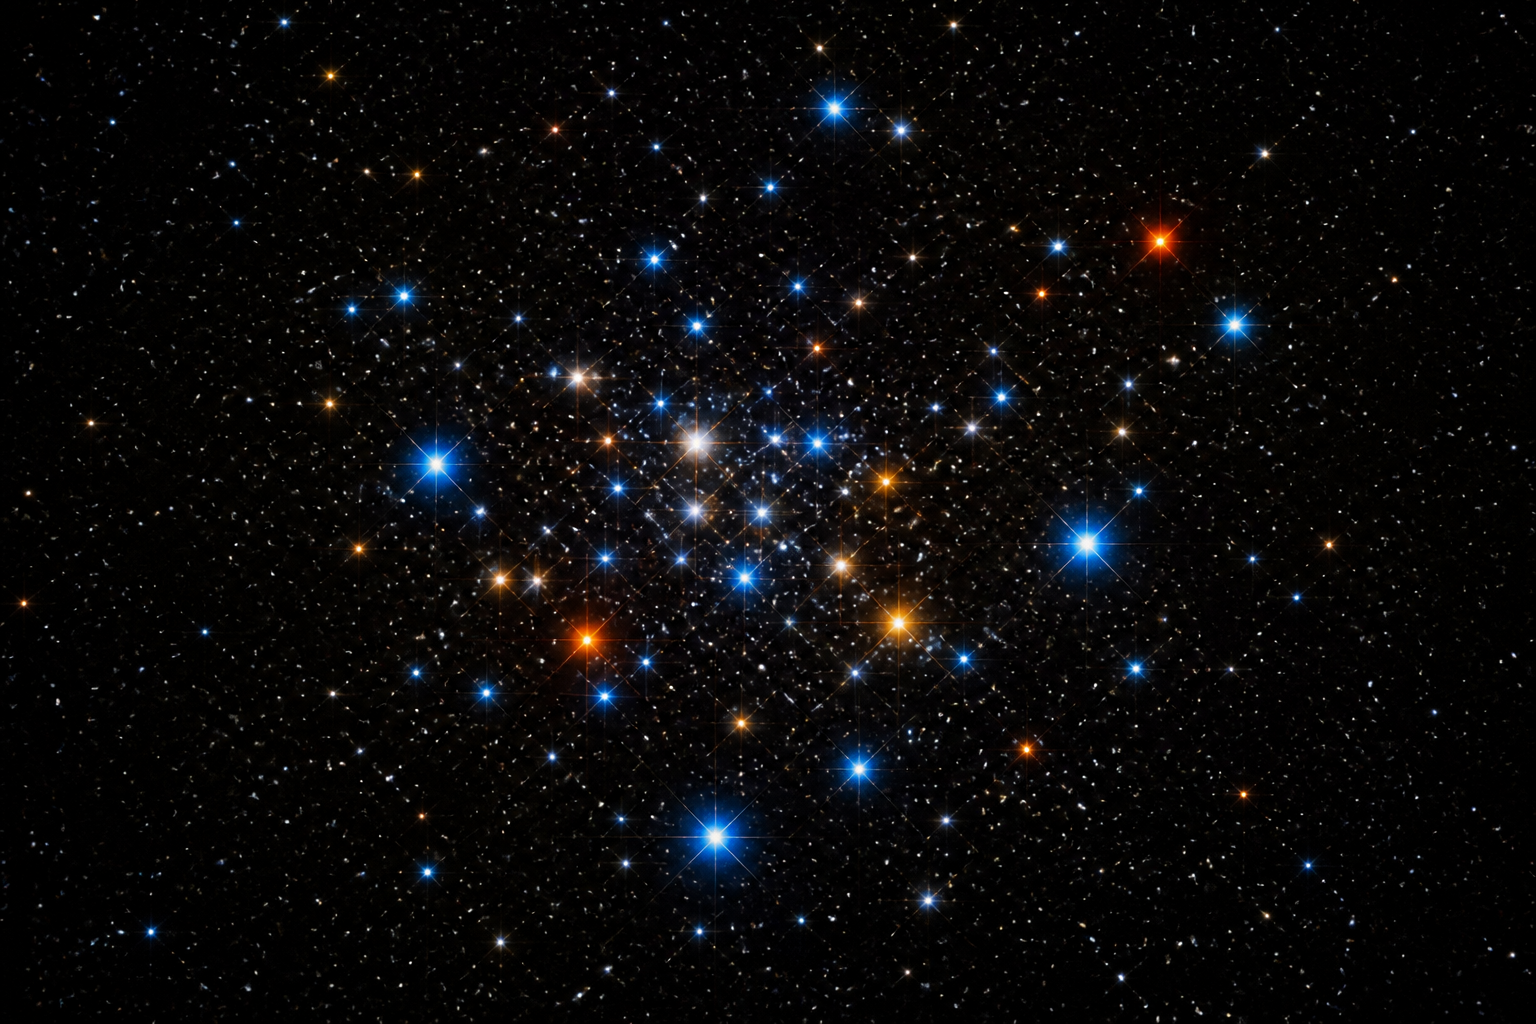
\includegraphics[width=0.58\linewidth]{images/book5/ai/b5-23-star-colors.png}

{\small Um aglomerado aberto: esbanjadoras branco-azuladas e anãs alaranjadas frugais, nascidas juntas, envelhecendo a ritmos muito diferentes --- o \omterm{def:b3:astrophysics:hr}{diagrama de Hertzsprung--Russell}, fotografado.}
\end{omfigure}

\section{Exercícios}

\begin{exercise}[$\star$]\label{exo:b3:astrophysics:1}
O Sol, estimado. $M = \qty{2e30}{kg}$, $R = \qty{7e8}{m}$.
(a) Estime $P_{\text{c}} \sim GM^2/R^4$. (b) Com a densidade
média e a lei dos gases ideais ($P = \rho k_{\text{B}}T/
m_{\text{p}}$), estime $T_{\text{c}}$. (c) Compare com o
limiar de ignição de $10^7\,\unit{K}$ do
\cref{exo:b3:nuclear-physics:11}. (d) Por que essa concordância é um
termostato, e não uma coincidência?
\end{exercise}

\begin{exercise}[$\star$]\label{exo:b3:astrophysics:2}
Pesando a luz. (a) A partir da constante solar
\qty{1360}{W/m^2} a $d = \qty{1.5e11}{m}$, calcule
$L_\odot$. (b) A partir de $L = 4\pi R^2\sigma T^4$, calcule a
temperatura superficial. (c) Confira o máximo de Wien contra o
amarelo-esverdeado visível do Sol. (d) Que lei de que capítulo cada passo usou?
\end{exercise}

\begin{exercise}[$\star$]\label{exo:b3:astrophysics:3}
Lendo o diagrama. Sirius B: $T \approx \qty{25000}{K}$, $L
\approx 0.026\,L_\odot$; Betelgeuse: $T \approx \qty{3500}{K}$,
$L \approx 10^5\,L_\odot$. (a) Situe as duas no diagrama HR. (b)
A partir de $L = 4\pi R^2\sigma T^4$, calcule cada raio em unidades
solares. (c) Betelgeuse no Sistema Solar: que planetas ficam
dentro dela? (d) O que tem de estar segurando Sirius B?
\end{exercise}

\begin{exercise}[$\star$]\label{exo:b3:astrophysics:4}
Viva rápido, morra jovem. Com $L \propto M^{3.5}$ e tempo de vida
$t \propto M/L$, e os dez bilhões de anos do Sol: (a) o tempo de vida
de uma estrela de $10\,M_\odot$; (b) o de uma anã vermelha de
$0.5\,M_\odot$ --- compare com a idade do universo; (c) por que as
estrelas mais pesadas, com \emph{mais} combustível, morrem \emph{antes}?
(d) O que a brevidade das vidas massivas implica sobre onde (numa
galáxia) ocorrem as supernovas?
\end{exercise}

\begin{exercise}[$\star\star$]\label{exo:b3:astrophysics:5}
A termodinâmica estranha da gravidade. Para uma bola de gás
autogravitante, o teorema do virial (\cref{ch:b3:lagrangian-mechanics})
dá energia total $E = -K$ (menos a energia cinética/térmica).
(a) Deduza: irradiar energia embora deixa a estrela \emph{mais quente}
--- uma capacidade térmica negativa. (b) Estime a energia
gravitacional $GM^2/R$ do Sol. (c) Ao $L_\odot$ de hoje, por quanto tempo
só a contração poderia tê-lo alimentado (o tempo de
Kelvin--Helmholtz)? (d) A geologia data a Terra em 4,5 bilhões de anos:
enuncie o paradoxo do século XIX e a resolução nuclear dele.
\end{exercise}

\begin{exercise}[$\star\star$]\label{exo:b3:astrophysics:6}
Anatomia de uma \omterm{ex:b3:quantum-statistics:dwarf}{anã branca}. Tome $M = 1\,M_\odot$ a
$R = R_{\text{Terra}} = \qty{6.4e6}{m}$. (a) Calcule a densidade
média e a massa de uma colher de chá (\qty{5}{mL}). (b) Calcule a
gravidade superficial. (c) A \omterm{thm:b3:quantum-statistics:fermi}{pressão de degenerescência} do
\cref{ch:b3:quantum-statistics} escala como $n^{5/3}$, e a exigência da
gravidade como $M^2/R^4 \propto n^{4/3}M^{2/3}$: mostre que isso implica
o bizarro $R \propto M^{-1/3}$ --- as anãs mais pesadas são
\emph{menores}. (d) Explique fisicamente por que empilhar massa
encolhe a estrela, e o que isso anuncia na \omterm{prop:b3:astrophysics:compact}{massa de
Chandrasekhar}.
\end{exercise}

\begin{exercise}[$\star\star$]\label{exo:b3:astrophysics:7}
Anatomia de uma \omterm{prop:b3:astrophysics:compact}{estrela de nêutrons}. (a) À densidade nuclear
$\qty{2.3e17}{kg/m^3}$, calcule o raio que segura
$1.4\,M_\odot$. (b) O núcleo pré-colapso girava uma vez a cada 25 dias
a $R \sim 10^5\,\unit{km}$: use a conservação do momento angular
para estimar o período final de rotação. (c) Calcule a gravidade
superficial. (d) O congelamento de fluxo amplifica o campo magnético como
$B \propto 1/R^2$ (\cref{ch:b3:electromagnetism-in-matter}):
a partir de \qty{e-2}{T} estelares, que campo superficial resulta, e
por que os pulsares emitem em feixe?
\end{exercise}

\begin{exercise}[$\star\star$]\label{exo:b3:astrophysics:8}
O ponto sem retorno. (a) Deduza $R_{\text{s}} = 2GM/c^2$ da
condição newtoniana de velocidade de escape $v_{\text{esc}} = c$ (a
dedução honesta precisa da relatividade geral; a resposta,
notoriamente, concorda). (b) Avalie para o Sol e para a Terra.
(c) O \omterm{prop:b3:astrophysics:compact}{buraco negro} central da Galáxia: $M = 4\times10^6\,M_\odot$
--- calcule $R_{\text{s}}$ e compare com a distância
Sol--Mercúrio ($\qty{5.8e10}{m}$). (d) Mostre que a densidade média dentro
de $R_{\text{s}}$ cai como $1/M^2$ --- um \omterm{prop:b3:astrophysics:compact}{buraco negro} grande o bastante é
menos denso que a água: o que isso diz sobre as intuições de
``esmagamento''?
\end{exercise}

\begin{exercise}[$\star\star\star$]\label{exo:b3:astrophysics:9}
Aritmética de Hubble. $H_0 = \qty{70}{km/s}$ por Mpc; $1\,
\text{Mpc} = \qty{3.09e22}{m}$. (a) Converta $H_0$ ao SI. (b)
Calcule $1/H_0$ em anos. (c) Uma galáxia a \qty{200}{Mpc}: a
velocidade de recessão dela e o fator pelo qual o comprimento de onda da
luz dela se esticou (Doppler de $z$ pequeno,
\cref{ch:b3:relativistic-kinematics}). (d) Por que $1/H_0$ é só
aproximadamente a idade do universo --- o que a taxa de expansão
andou fazendo nesse meio-tempo?
\end{exercise}

\begin{exercise}[$\star\star\star$]\label{exo:b3:astrophysics:10}
A luz mais antiga. A CMB é um corpo negro a \qty{2.725}{K}. (a)
Calcule o comprimento de onda de máximo dela (\cref{ch:b3:photons-phonons}) e
justifique o ``micro-ondas''. (b) Ela foi emitida como
luz de \qty{3000}{K}: que fator de expansão a esticou,
e por que \qty{3000}{K} (lembre Saha,
\cref{prop:b3:grand-canonical:saha})? (c) A densidade de fótons dela é
$\sim\qty{4e8}{m^{-3}}$: compare com a densidade de \omterm{def:b3:particle-physics:zoo}{bárions},
$\sim\qty{0.25}{m^{-3}}$, e enuncie a razão \omterm{def:b3:particle-physics:zoo}{fóton-bárion}.
(d) Uma verificação clássica de mesa: alguns por cento da estática de uma
TV analógica fora de sintonia eram a CMB --- por que uma antena, apontada
para onde for, a recebe?
\end{exercise}

\begin{exercise}[$\star\star\star$]\label{exo:b3:astrophysics:11}
Um quarto de hélio, de um fator de Boltzmann. Por volta de $t \sim
\qty{1}{s}$, $T \sim \qty{e10}{K}$ ($k_{\text{B}}T \approx
\qty{0.8}{MeV}$), as reações fracas ao congelarem deixaram a
razão nêutron-próton no valor de Boltzmann dela
(\cref{ch:b3:canonical-ensemble}). (a) Com $\Delta mc^2 =
\qty{1.29}{MeV}$, calcule $n/p$ no congelamento. (b) O decaimento de
nêutrons nos primeiros minutos a aparou para $\approx1/7$: mostre que
ligar cada sobrevivente em $^4$He dá uma fração de \emph{massa} de hélio
de $2(n/p)/(1 + n/p) = 25\,\%$. (c) Diga por que esse número,
medido em estrelas de toda parte, é evidência poderosa do começo
quente. (d) Por que a cozinha primordial parou no hélio
(com traços de lítio), deixando o carbono e todo o resto para a
\cref{rem:b3:astrophysics:evolution}?
\end{exercise}

\begin{exercise}[$\star\star\star$]\label{exo:b3:astrophysics:12}
A matéria que falta. A velocidade de rotação de uma galáxia espiral fica
plana em $v = \qty{220}{km/s}$ até $r = \qty{50}{kpc}$
($\qty{1.5e21}{m}$), bem além da borda visível dela. (a) Para uma
órbita circular, mostre que $M(r) = v^2r/G$. (b) Avalie em
\qty{50}{kpc}, em massas solares. (c) As estrelas e o gás visíveis
totalizam $\sim5\times10^{10}\,M_\odot$: que fração fica
explicada? (d) A expectativa kepleriana além da borda visível
é $v \propto r^{-1/2}$ (o padrão do Sistema Solar): o que a
planura implica sobre como a massa invisível se distribui?
\end{exercise}

\begin{omfigure}
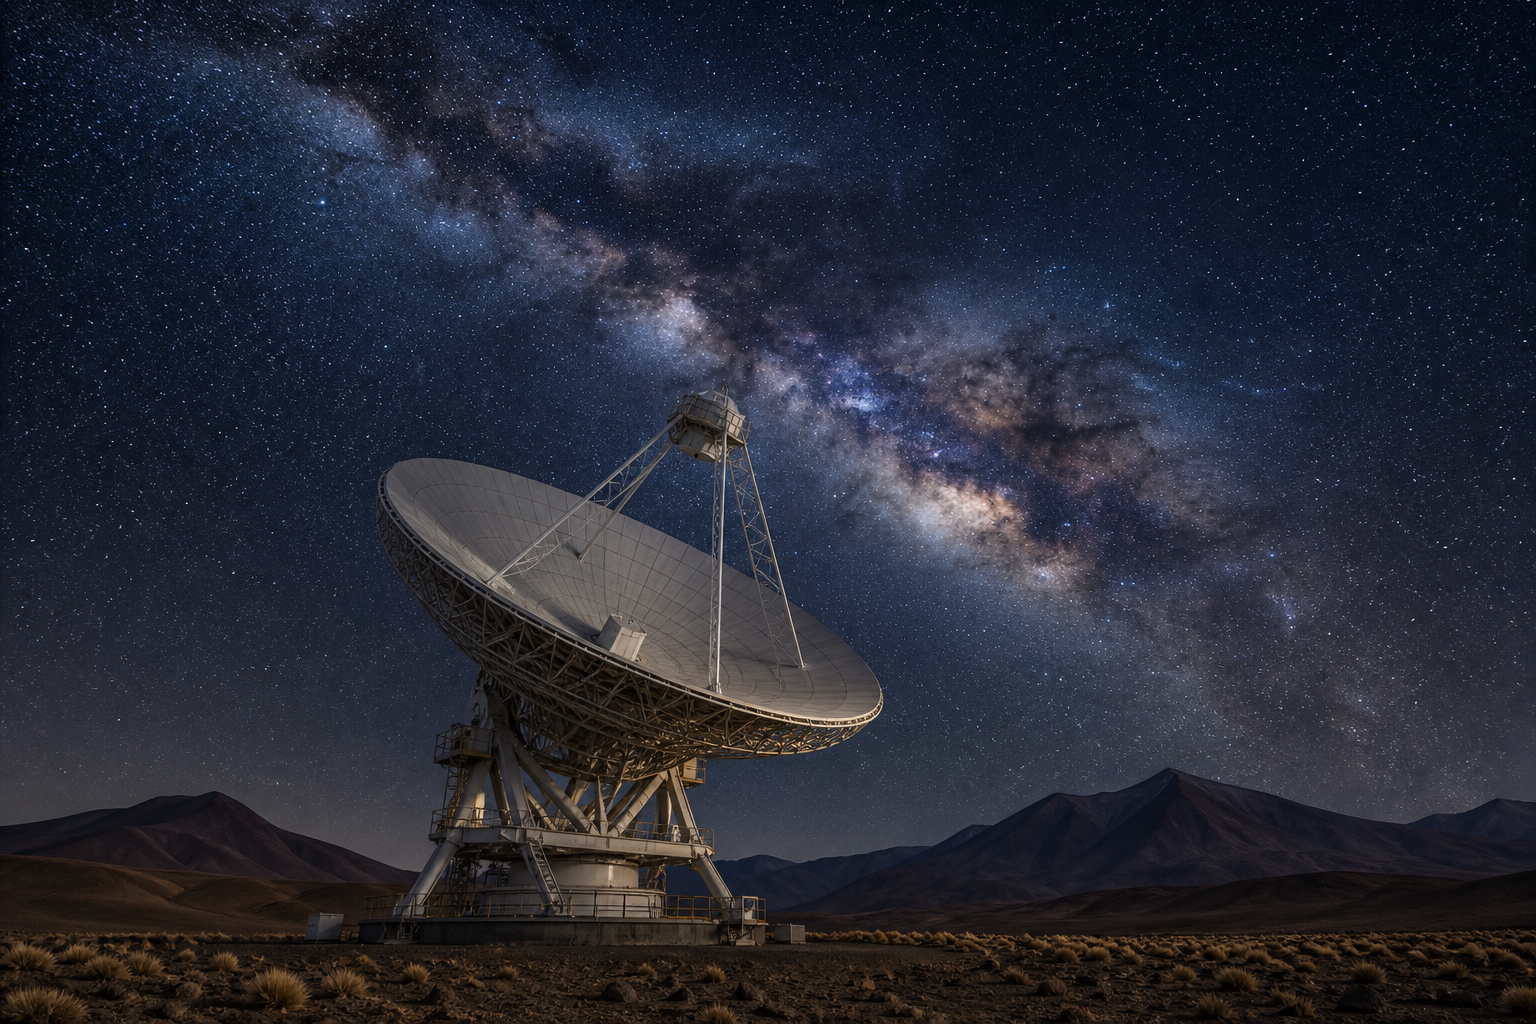
\includegraphics[width=0.58\linewidth]{images/book5/ai/b5-10-radio-dish.png}

{\small Uma antena de ondas milimétricas sob a Via Láctea: a galáxia que ela escuta, pairando acima dela. A radioastronomia achou a \omterm{def:b3:astrophysics:hubble}{radiação cósmica de fundo em micro-ondas} --- o chiado a \qty{2.7}{K} que acabou sendo o começo.}
\end{omfigure}

\begin{omfigure}
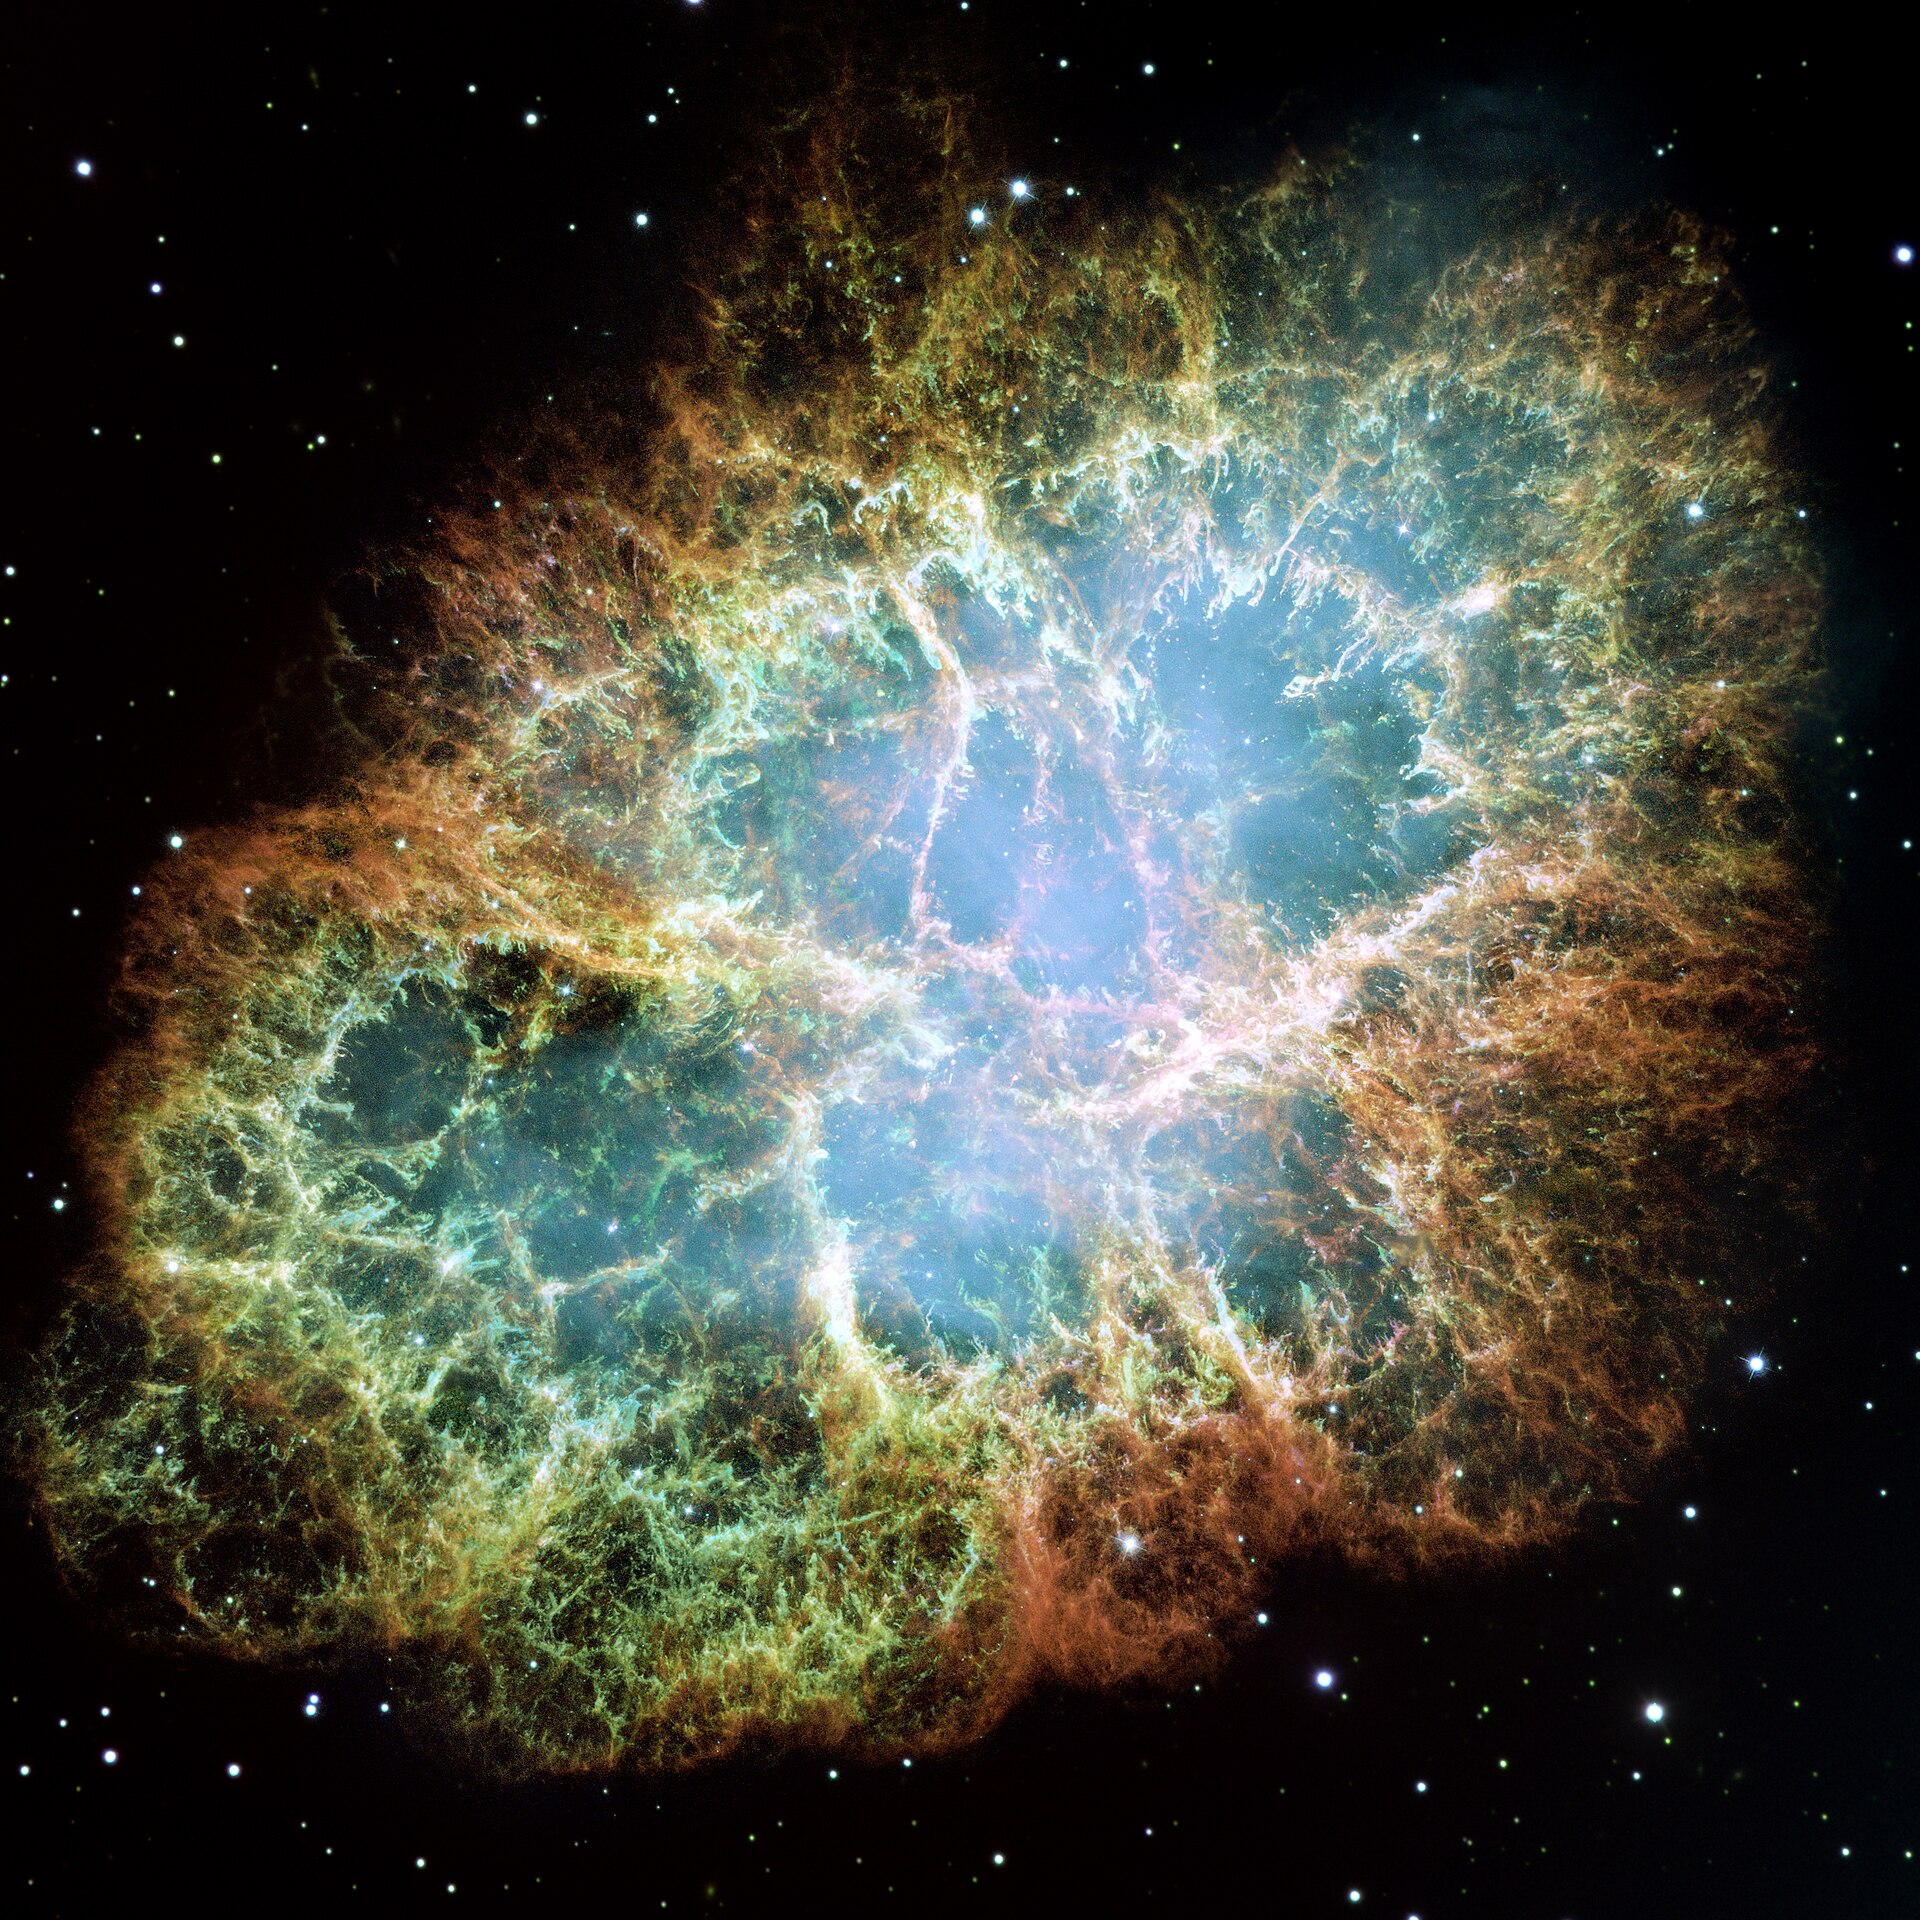
\includegraphics[width=0.6\linewidth]{images/book5/photo-crab-nebula.jpg}

{\small A nebulosa do Caranguejo (NASA, ESA, J. Hester e A. Loll, domínio público): os destroços da supernova de 1054, ainda em expansão, com o farol de milissegundos de uma \omterm{prop:b3:astrophysics:compact}{estrela de nêutrons} no coração dela --- o problema de fim de semana, fotografado nove séculos depois.}
\end{omfigure}

\section{Problema: a noite em que a estrela morreu}

\begin{problem}\label{pb:b3:astrophysics:1}
\emph{A noite em que a estrela morreu.} Em 23 de fevereiro de 1987, uma
supergigante azul da Grande Nuvem de Magalhães --- $d \approx
\qty{50}{kpc} \approx \qty{1.5e21}{m}$ --- virou a SN~1987A, a
supernova mais próxima em quatro séculos. Horas \emph{antes} de qualquer
telescópio vê-la brilhar, três detectores subterrâneos contaram
duas dúzias de neutrinos. Você vai reconstruir aquela noite a partir de
primeiros princípios.

\medskip\noindent\textbf{Parte I --- A estrela que existia.}

\begin{enumerate}
  \item A progenitora pesava ${\sim}20\,M_\odot$. Usando
        a escala do \cref{exo:b3:astrophysics:4}, estime o
        tempo de vida dela e compare com o do Sol.
  \item No último dia dela, a estrela era uma cebola: cascas de H, He, C,
        O e Si em torno de um núcleo de ferro. Por que cada
        combustível seguinte exige um núcleo mais quente?
  \item Por que a sequência para, em definitivo, no ferro?
        (\cref{prop:b3:nuclear-physics:binding}.)
  \item O núcleo inerte de ferro cresce rumo a $1.4\,M_\odot$. O que
        há de especial nesse número, e que pressão falha
        ali?
  \item A queima do silício sustenta a estrela por cerca de um
        \emph{dia}: o que isso diz sobre como o relógio de uma
        estrela acelera rumo ao fim?
  \item Uma vez que o sustento por pressão falha, quanto tempo dura
        aproximadamente a queda livre, para um núcleo de densidade
        $\sim\qty{e12}{kg/m^3}$ ($t \sim 1/\sqrt{G\rho}$)?
\end{enumerate}

\medskip\noindent\textbf{Parte II --- O clarão de neutrinos.}

\begin{enumerate}[resume]
  \item O núcleo ($M \approx 1.4\,M_\odot = \qty{2.8e30}{kg}$)
        desaba até $R \approx \qty{12}{km}$: calcule a
        energia gravitacional liberada, $E \sim GM^2/R$.
  \item Compare com a luz de um bilhão de sóis brilhando por um
        mês ($L \sim 10^{9}L_\odot$ por $\qty{2.6e6}{s}$):
        mostre que os fótons são erro de arredondamento --- para onde vão
        os 99\,\%, e por que só os neutrinos conseguem escapar de pronto
        de um núcleo em colapso?
  \item Espalhe $E \approx \qty{3e46}{J}$ por uma esfera de
        raio \qty{1.5e21}{m}: calcule a fluência de energia na
        Terra.
  \item Com $\sim\qty{15}{MeV}$ por neutrino, calcule a
        fluência de número (neutrinos por \unit{m^2}).
  \item Um detector guarda \qty{2000}{t} de água:
        ${\sim}1.5\times10^{32}$ prótons livres. Com uma
        probabilidade de interação por próton de
        $\sigma \approx \qty{1e-46}{m^2}$ por antineutrino
        (dada), estime a contagem esperada --- e compare
        com os onze que um detector registrou.
  \item Os neutrinos venceram a luz por horas. Explique os dois
        relógios: o que atrasa os fótons (onde o
        aumento de brilho nasce, de fato?) e o que a
        quase \omterm{def:b3:relativistic-kinematics:event}{simultaneidade} diz sobre a massa e a
        velocidade do neutrino?
  \item Vinte e cinco neutrinos contados: diga, em uma frase
        cada, duas coisas que eles confirmaram sobre a teoria das supernovas.
\end{enumerate}

\medskip\noindent\textbf{Parte III --- O que resta.}

\begin{enumerate}[resume]
  \item Calcule a densidade média do remanescente de \qty{12}{km} e
        $1.4\,M_\odot$ e compare com a densidade nuclear da
        \cref{def:b3:nuclear-physics:nuclide}.
  \item O núcleo progenitor girava uma vez a cada 30 dias a
        $R \sim \qty{e5}{km}$: estime o período do remanescente.
  \item O campo magnético dele, congelado no fluxo, é amplificado por
        $(R_0/R)^2$: a partir de \qty{e-2}{T}, calcule o campo
        superficial.
  \item Explique o farol: o que varre, o que emite em feixe e
        por que o pulsar do Caranguejo (nascido em 1054, cronicado como uma
        ``estrela visitante'' diurna) ainda pisca trinta vezes por segundo.
  \item Se o remanescente tivesse passado de ${\sim}3\,M_\odot$: calcule
        $R_{\text{s}}$ para $3\,M_\odot$ e diga o destino dele.
  \item A temporização dos pulsares é estável a $10^{-15}$: cite um uso
        físico de um relógio tão bom, girando no céu.
\end{enumerate}

\medskip\noindent\textbf{Parte IV --- O que isso significa.}

\begin{enumerate}[resume]
  \item O oxigênio que você respira e o ferro do seu sangue:
        trace a biografia de cada átomo em duas frases, do
        hidrogênio do Big Bang à sua corrente sanguínea.
  \item As supernovas de tipo Ia (\omterm{ex:b3:quantum-statistics:dwarf}{anãs brancas} empurradas para além de
        $M_{\text{Ch}}$) detonam todas na mesma massa, e portanto
        com quase o mesmo brilho. Explique por que isso as torna
        \emph{velas-padrão}, e como o diagrama da
        \cref{def:b3:astrophysics:hubble} é construído
        a partir delas.
  \item Em 1998, supernovas Ia distantes saíram \emph{mais fracas}
        do que a reta de Hubble prevê: enuncie a
        conclusão que ganhou o Nobel de 2011.
  \item Estime que distância a luz da SN~1987A havia percorrido quando
        chegou, em anos --- e note o que acontecia na
        Terra quando ela partiu.
  \item Os neutrinos da LMC atravessaram você também (todos os que
        estavam vivos naquele dia). Grosso modo, quantos cruzaram cada ser
        humano (${\sim}\qty{0.03}{m^2}$)? Alguém sentiu
        (\cref{exo:b3:particle-physics:10})?
  \item Feche o livro-caixa do livro em quatro linhas: uma estrela
        equilibrada por dez milhões de anos pelo tunelamento; um colapso
        pago em neutrinos; um cadáver sustentado por Pauli; e os
        destroços --- inclusive o leitor --- ainda cavalgando
        a expansão de Hubble.
\end{enumerate}
\end{problem}
